% You should title the file with a .tex extension (hw1.tex, for example)
\documentclass[11pt]{article}

\usepackage{hyperref}
\usepackage{amsmath}
\usepackage{mathtools}
\usepackage{amssymb}
\usepackage{wrapfig}
\usepackage{fancyhdr}
\usepackage{tikz-qtree}
\usepackage{tikz-qtree-compat}
\usepackage[normalem]{ulem}
\usepackage{tikz}
\usepackage{graphicx}
\DeclareMathOperator*{\argmin}{argmin}
\DeclareMathOperator*{\argmax}{argmax}

\oddsidemargin0cm
\topmargin-2cm     %I recommend adding these three lines to increase the 
\textwidth16.5cm   %amount of usable space on the page (and save trees)
\textheight23.5cm  

\newcommand{\question}[2] {\vspace{.25in} \hrule\vspace{0.5em}
\noindent{\bf #1: #2} \vspace{0.5em}
\hrule \vspace{.10in}}
\renewcommand{\part}[1] {\vspace{.10in} {\bf (#1)}}

\newcommand{\myname}{Sean Bittner}
\newcommand{\myandrew}{srb2201@columbia.edu}
\newcommand{\myhwnum}{12}

\setlength{\parindent}{0pt}
\setlength{\parskip}{5pt plus 1pt}
 
\DeclarePairedDelimiter\abs{\lvert}{\rvert}%
 %
\pagestyle{fancyplain}
\rhead{\fancyplain{}{\myname\\ \myandrew}}

\begin{document}

\medskip                        % Skip a "medium" amount of space
                                % (latex determines what medium is)
                                % Also try: \bigskip, \littleskip

\thispagestyle{plain}
\begin{center}                  % Center the following lines
{\Large Draft of new V1 section} \\
Sean Bittner, Agostina Palmigiano \\
October 6, 2020 \\
\end{center}

\section{EPI clarifies the implications of contrast-response flipping on [noise quenching, inhibition stabilization] in V1}\label{results_V1}
Dynamical models of excitatory (E) and inhibitory (I) populations with supralinear input-output function have succeeded in explaining a host of experimentally documented phenomena.
In a regime characterized by inhibitory stabilization of strong recurrent excitation, these models give rise to paradoxical responses \cite{tsodyks1997paradoxical}, selective amplification  \cite{murphy2009balanced}, surround suppression \cite{ozeki2009inhibitory} and normalization \cite{rubin2015stabilized}. 
Despite their strong predictive power, E-I circuit models rely on the assumption that inhibition can be studied as an indivisible unit. 
However, experimental evidence shows that inhibition is composed of distinct elements -- parvalbumin (P), somatostatin (S), VIP (V) --
composing 80\% of GABAergic interneurons in V1 \cite{markram2004interneurons, rudy2011three, tremblay2016}, and that these inhibitory cell types follow specific connectivity patterns (Fig. \ref{fig:SV_flip}A) \cite{pfeffer2013inhibition}.
Recent theoretical advances \cite{litwin2016inhibitory, GarciaDelMolino2017, Chen2019},  have only started to address the consequences of this multiplicity in the dynamics of V1, strongly relying on linear theoretical tools. 
Here, we use EPI to analyze the posteriors of a stochastic nonlinear dynamical model of V1 conditioned on the emergent property of contrast-dependent S-V flipping.
We then [use this info to make a statement about ...]

Specifically, we consider a four-dimensional circuit model with dynamical state given by the firing rate $x$ of each neuron-type population $x = \left[x_E, x_P , x_S, x_V \right]^\top$. Given a time constant of $\tau = 20$ ms and a power $n = 2$, the dynamics are driven by the rectified and sum of recurrent inputs $Wx$, external inputs $h$, and external noise $\epsilon \sim \mathcal{N}(0, \sigma_{\epsilon}^2)$:

\begin{equation}
\tau \frac{dx}{dt} = -x + [W x+ h + \epsilon]_+^n.
\end{equation}

We considered fixed effective connectivity weights $W$ approximated from experimental recordings of publicly available datasets of mouse V1 \cite{allen2018layer, billeh2019systematic} (see Section \ref{methods_V1}).
The input $h = b + dh$ is comprised of a baseline input  $b = \left[ b_E, b_P , b_S , b_V \right]^\top$ and a differential input $dh = \left[ dh_E , dh_P , dh_S , dh_V\right]^\top$ to each neuron-type population.  
Throughout subsequent analyses, the baseline input is $b = \left[ 1 ,1,1,1\right]^\top$. 

With this model, we are interested in the differential responses of each neuron-type population to changes in input $dh$. 
Initially, we studied the linearized response of the system to input $\frac{dx_{ss}}{dh}$ at the steady state response $x_{ss}$, i.e. a fixed point. 
All analyses of this model consider the steady state response, so we drop the notation $ss$ from here on.
While this linearization accurately predicts differential responses $dx = \left[ dx_{E} , dx_{P} , dx_{S} ,dx_{V} \right]^\top$  for small differential inputs to each population $dh = \left[ 0.1 , 0.1 , 0.1 , 0.1 \right]^\top$ (Fig \ref{fig:V1_EPI}B left), the linearization is a poor predictor in this nonlinear model more generally (Fig. \ref{fig:V1_EPI}B right).  
Currently available approaches to deriving the steady state response of the system are limited.

\clearpage
\begin{figure}[h]
\caption{\small \textbf{A}.  Four-population model of primary visual cortex with excitatory (black), parvalbumin (blue), somatostatin (red), and VIP (green) neurons.   Some neuron-types largely do not form synaptic projections to others  (excitatory and inhibitory projections filled and unfilled, respectively).
\textbf{B}. EPI posterior $q_\theta(z \mid \mathcal{B}_{S-V})$ for S-V flipping. The obtained posterior is visualized as 500 samples from the inferred distribution colored by $\log(q_\theta(z))$. This posterior is bimodal and concentrated in planes $dh_E > 0$ and $dh_E < 0$ at distinct modes $z_1$ (black star) and $z_2$ (gray, star), respectively.  Bottom-left: Posterior predictive distribution of the emergent property statistics with respect to the constrained means (black, dashed line) and variances (gray, dashed lines at two stds). 
\textbf{C}. Posterior predictive distribution of $d_{S-V}(h)$ of each mode shows that the $z_1$-mode produces V-to-S flipping with increasing contrast and the $z_2$-mode produces S-to-V flipping.
\textbf{D}. Model simulations at the mode $z_1$ at $b_1$ (left), $b_1 + dh_1^{(c)}$ (middle), and steady state solutions for varying levels of contrast (right).  Shaded area is one standard deviation according to randomness of $\epsilon$.  \textbf{E}. Same as D. for $z_2$. \textbf{F}. ...
 }\label{fig:SV_flip}
\begin{center}
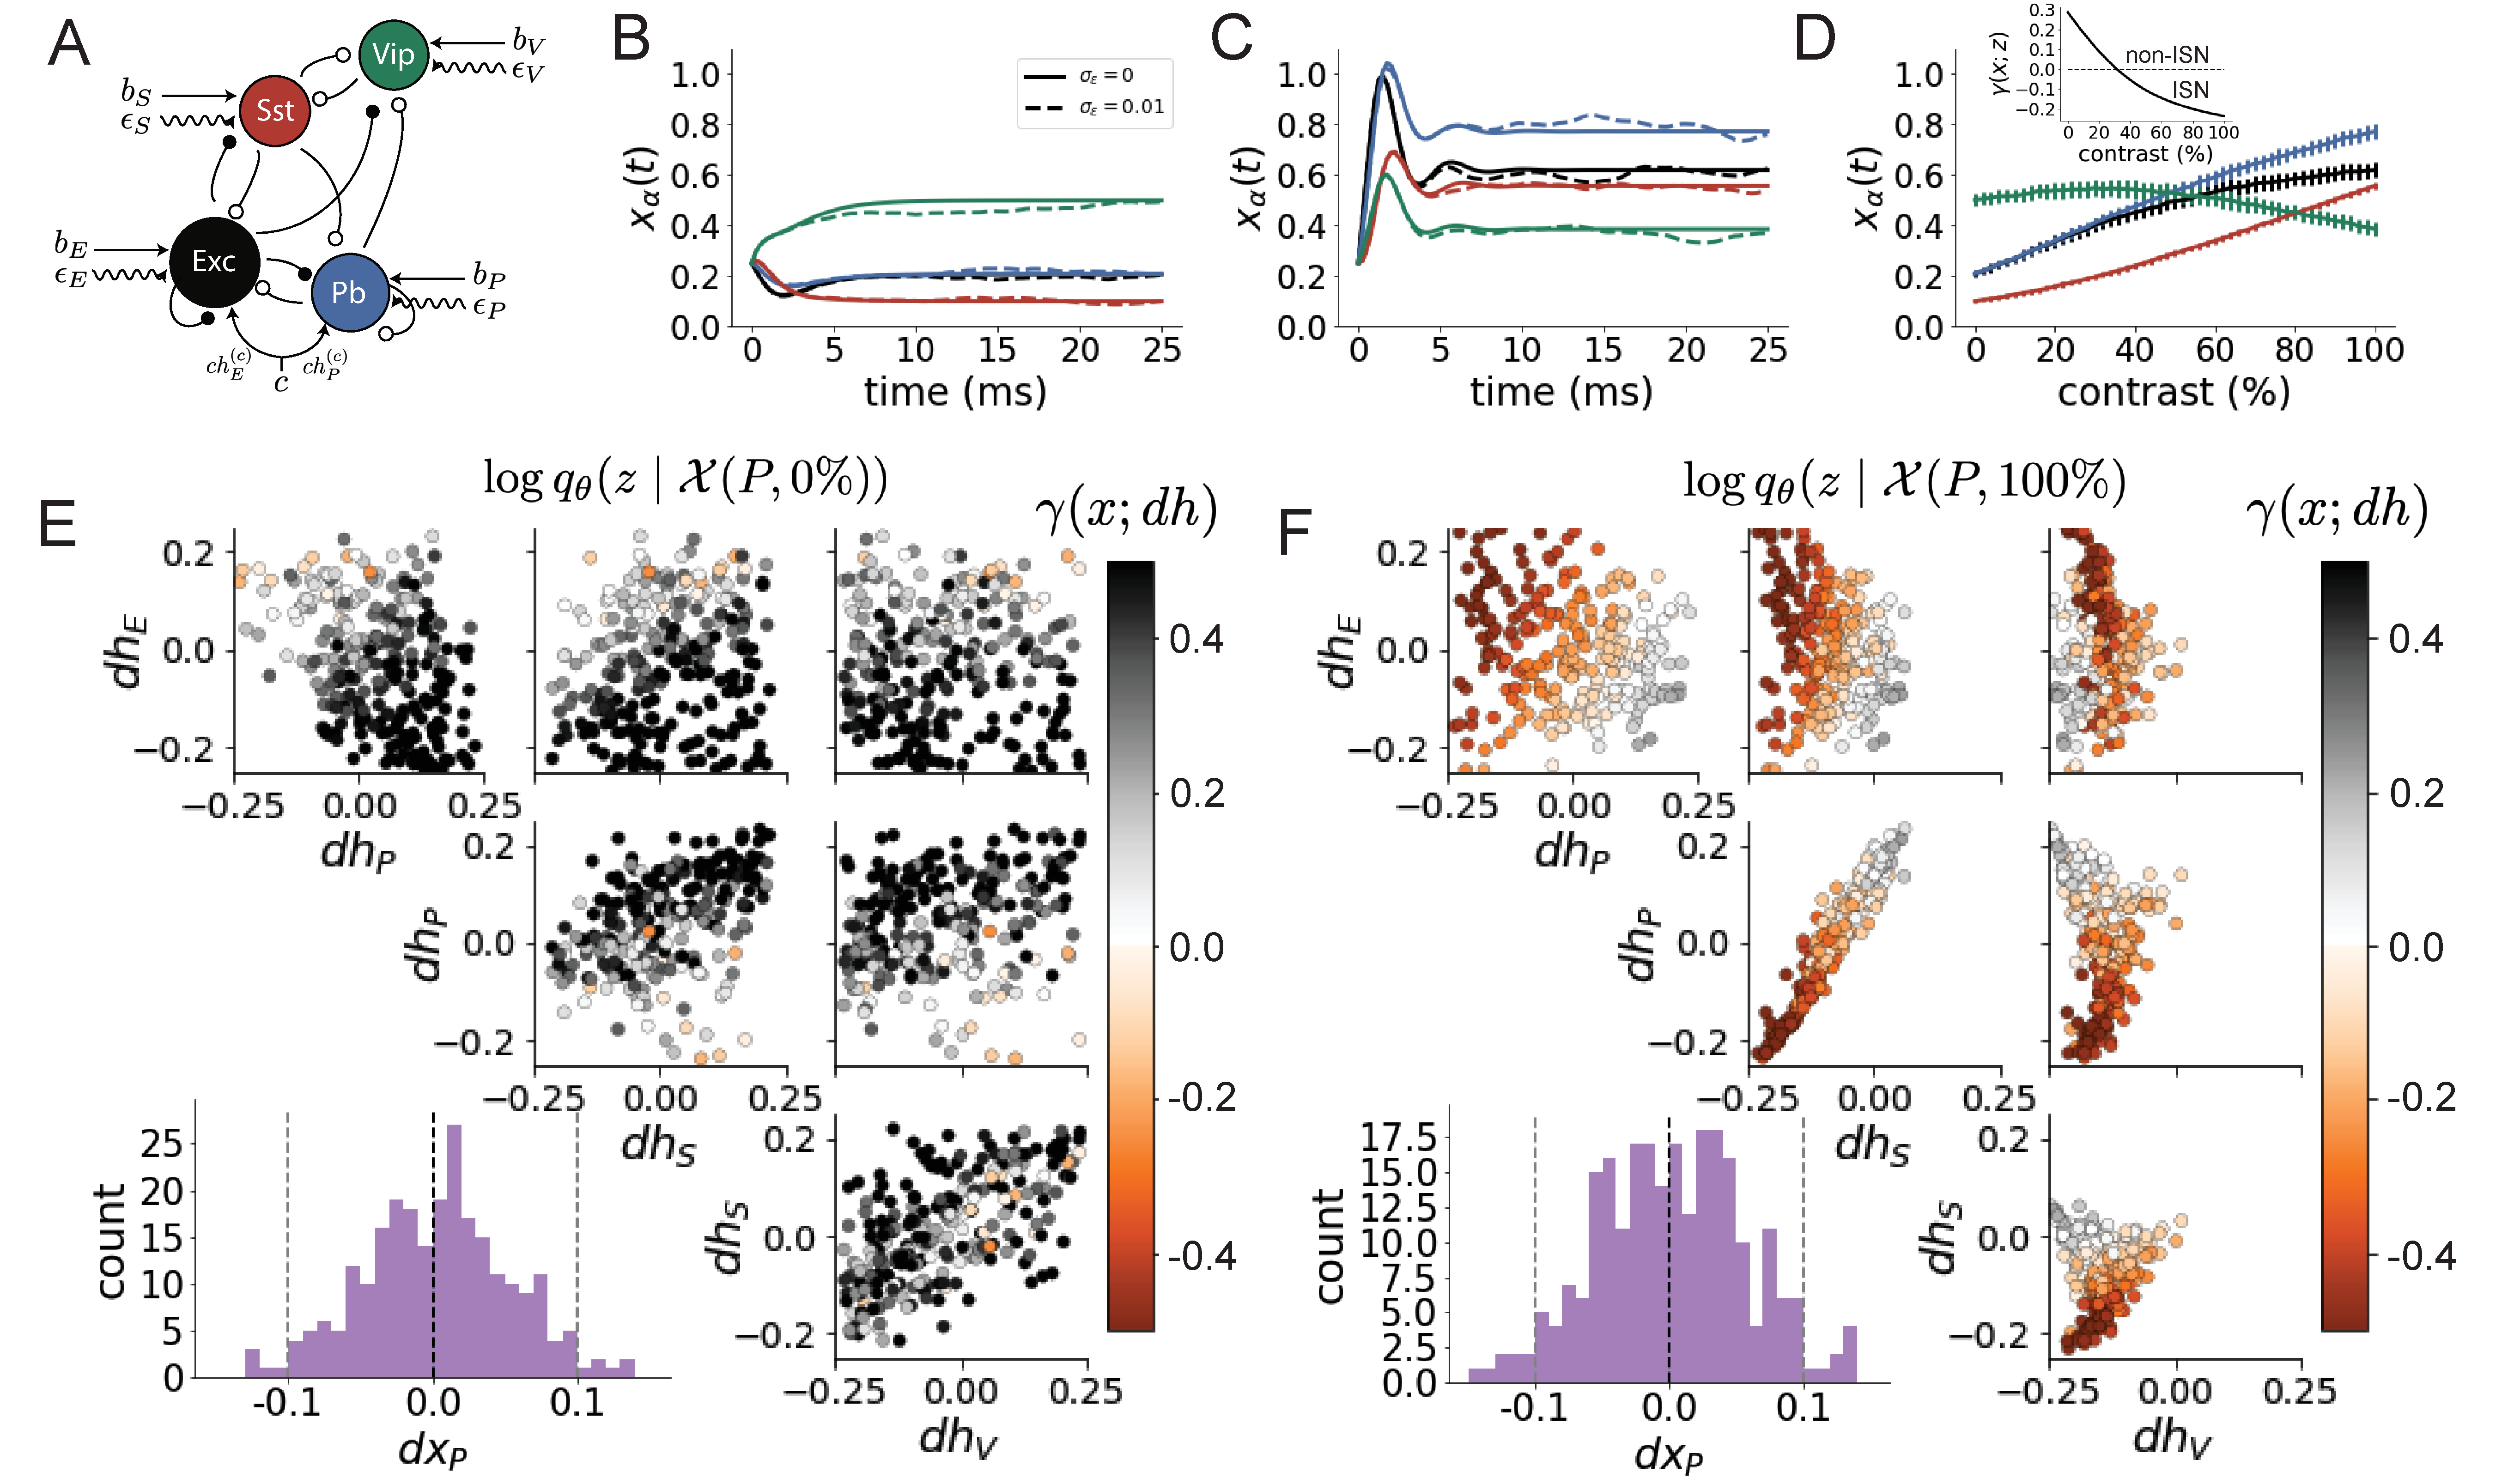
\includegraphics[scale=.31]{figs/Fig3/Fig3.pdf}
\end{center}
\end{figure}
\clearpage

TODO Summarize S-V flipping phenomena and why it's a good EP
TODO Explain that we can't really fit the whole data-set of responses yet because the model is quite constrained.
TODO Motivate this input model, where $dh^{(c)}$ is the direction of increasing contrast.

\begin{equation}
 \begin{bmatrix} h_E \\ h_P \\ h_S \\ h_V \end{bmatrix} =  \begin{bmatrix} b_E \\ b_P \\ b_S \\ b_V \end{bmatrix} +  \begin{bmatrix} dh^{(c)}_E \\ dh^{(c)}_P \\ 0 \\ 0 \end{bmatrix} 
\end{equation}

Since we are unsure what either the baseline input $b$ and contrast-dependent change in input $dh^{(c)}$ should be, we treat them as free parameters when running EPI.
\begin{equation}
 z =  \begin{bmatrix} b_E & b_P & b_S & b_V & dh^{(c)}_E & dh^{(c)}_P \end{bmatrix}^\top
\end{equation}
We consider positive baseline inputs $b_\alpha \in \left[0, 3 \right]$ and small contrast-dependent changes in input $|dh_\alpha| \leq 1$.  
To find parameters resulting in S-V flipping, we focus on models driven by nominal amounts of external noise $\sigma_{\eta} = 0.1$. 

We formulate the emergent property of S-V flipping with a statistic measuring he difference in steady state ($x_ss$) between the S- and V-population at a given input:
\begin{equation}
d_{S-V}(h) = x_{ss,S}(h) - x_{ss,V}(h).
\end{equation}
For S and V to flip their steady states, the difference between the S- and V-population rates at $h = b$ must have opposite sign from $h = b + dh$.  Therefore, we stipulate the emergent property of S-V flipping to require the product between $d_{S-V}(b)$ and $d_{S-V}(b+dh)$ to be appreciably negative.  Second we stipulate that the differences between S and V in each input condition cancel out on average ($d_{S-V}(b) + d_{S-V}(b+dh)$ is 0 on average).  The means and variances of the emergent property statistics were sensibly chosen based on some inexpensive model simulations within the parameter bounds.

\begin{equation}
\mathcal{B}_{S-V} \triangleq \mathbb{E}\begin{bmatrix} d_{S-V}(b)d_{S-V}(b+dh) \\ \left( d_{S-V}(b)d_{S-V}(b+dh) - (-0.25) \right)^2 \\  d_{S-V}(b) + d_{S-V}(b+dh) \\  \left( d_{S-V}(b) + d_{S-V}(b+dh)\right)^2 \end{bmatrix} = 
\begin{bmatrix} -0.25 \\ 0.125^2 \\ 0 \\ 0.125^2 \end{bmatrix}
\end{equation}

We ran EPI to inspect the structure of the posterior distribution of $z$ conditioned on S-V flipping shown in Fig 2.  
It is clear from this visualization that S-V flipping in this V1-model is sensitive with respect to some parameter settings and robust with respect to others.
Additionally, the posterior is bimodal: there is one mode in each of the hyperplanes $dh_E < 0$ and $dh_E > 0$.

The structure of the V1 model S-V flipping posterior yields the following insights:
\begin{enumerate}
\item The marginal distributions of $q_\theta(h_P \mid \mathcal{B}_{S-V})$ and  $q_\theta(dh_P \mid \mathcal{B}_{S-V})$ are approximately uniform along their allowed range.  
The approximate uniformity of the $P-population$ parameter marginal distributions shows that the P-population plays little role in S-V flipping. 
\item The pairwise marginal distribution of $q_\theta(h_S, h_V \mid \mathcal{B}_{S-V})$ shows strong correlation between these parameters.
The strong correlation between $h_S$ and $h_V$ in the posterior reveals that S-V flipping is sensitive with respect to the baseline inputs to the S- and V-populations.
\textbf{Augment this to show that multidim info from Hessian is useful.}
The Hessian provided by EPI at the modes indicates that coordinated increases of $h_S$ and $h_V$ by a ratio of $\frac{h_S}{h_V} = 0.701$ will preserve S-V flipping, while changes in an orthogonal dimension will disrupt it.

\item This distribution is multimodal.
\end{enumerate}

%\section{Stability analysis}
%The input $h = b + dh$ is comprised of a baseline input  $b = \left[ b_E, b_P , b_S , b_V \right]^\top = \left[ 1, 1, 1 ,1.25 \right]^\top$  and a differential input $dh = \left[ dh_E , dh_P , dh_S , dh_V\right]^\top$ to each neuron-type population.  
%
%We want to know the differential inputs $dh$ that maintain the steady state $x_{\alpha}$ for $\alpha \in \{E, P, S, V\}$. 
%We see from Figure 1B that input to a single population in the recurrent circuit elicits a variety of responses across populations: E same, P up, S down, and V up.
%We define the differential steady state $dx_{\alpha}$ as the change in steady state $x_{\alpha}$ when receiving input $h=b + dh$ with respect to the baseline $h = b$.
%Maintaining the steady state of a neuron-type population amounts to the emergent property 
%\begin{equation}
%\mathcal{B}(\alpha, \sigma) ~~\triangleq~~ 
%\mathbb{E} \begin{bmatrix} dx_{\alpha} \\ dx_{\alpha}^2 \end{bmatrix} ~~=~~ \begin{bmatrix} 0 \\ \sigma^2 \end{bmatrix}.\\
%\end{equation}
%In the following analyses, we chose $\sigma=0.25$.
%
%\section{EPI agrees with ABC}
%To get an idea of what distribution of parameters ($dh$) we should expect from EPI, we can use ABC to obtain a set of parameters related to the emergent property.  
%We compare EPI to ABC with a rejection heuristic defined by the standard deviation of the differential responses $\sigma_{ABC}$
% \[f_{ABC}(dx_\alpha; \sigma_{ABC}) = |dx_\alpha| > 2\sigma_{ABC}.\]
% In other words, we ran ABC accepting parameters that generate differential responses within two standard deviations $\sigma_{ABC}=0.25$ of $dx_\alpha = 0$.
% In Figure 2, we see that the distributions obtained via EPI (colored by $\log q_\theta(z)$) are visually similar to those obtained via ABC (colored by $dx_\alpha$). \\
% 
% \textbf{Figure 2}: EPI (left) vs ABC (right).  Arrows in EPI distribution indicate dimensions of maximal sensitivity at selected parameters $dh$. The importance of $v_S$ and $v_P$ are explained in section 4.2. \\
%
%There are some subtle differences between the EPI and ABC distributions, but some difference is to be expected.
%Rather than simply attributing these differences to imperfection of the EPI optimization routine, we consider the the effect of bias in $dx_\alpha$ from ABC (and lack thereof from EPI).
%
%When $\epsilon > 0$ in ABC, the samples are \textit{not} from the posterior distribution.
%For $\epsilon > 0$, the ``posterior" predictive means of ABC $\mathbb{E}_{ABC(\alpha, \sigma_{ABC})}\left[dx_\alpha \right]$ may be far from zero.
%In Figure 3, we see that with ABC, there is an increasingly negative bias in $\mathbb{E}_{ABC(\alpha, \sigma_{ABC})}\left[dx_\alpha \right]$ for greater error tolerances across all neuron-types.  
%Additionally with ABC, there is no precise control of the variance $\mathbb{E}_{ABC(\alpha, \sigma_{ABC})}\left[dx_\alpha^2 \right]$, which may be undesireable.
%
%In contrast, the first and second moments of $dx_\alpha$ are controlled to a specified degree of accuracy (Figure 4).
%The variances of each distribution of $dx_\alpha$ are close to their target value $0.25^2 = 0.0625$ (see variances next to histograms of Figure 4). 

\section{V1 Supplemental section}\label{methods_V1}
 
We considered fixed effective connectivity weights $W$ approximated from experimental recordings of publicly available datasets of mouse V1.  Specifically, Billeh et al. \cite{billeh2019systematic} produce estimates of the synaptic strength (in mV)
\begin{equation}
M = \begin{bmatrix} 
0.36 & -0.48 & -0.31 & -0.28 \\
1.49 & -0.68 & -0.50 & -0.18 \\
0.86 & -0.42 & -0.15 & -0.32 \\
1.31 & -0.41 & -0.52 & -0.37 \end{bmatrix}
\end{equation}
and connection probability
\begin{equation}
C = \begin{bmatrix} 0.16 & 0.411 & 0.424 &  0.087 \\
0.395 & .451 & 0.857 & 0.02 \\
0.182 & 0.03 & 0.082 & 0.625 \\
0.105 & 0.22 & 0.77 & 0.028 \end{bmatrix}.
\end{equation}

Multiplying these connection probabilities and synaptic efficacies gives us an effective connectivity matrix:
\begin{equation}
W = C \odot M = \begin{bmatrix} 
0.0576 & -0.197 & -0.131 & -0.0244 \\
0.589 & -0.307 & -0.429 & -0.00360 \\
0.157 & -0.0126  & -0.0123 & -0.200 \\
0.138 & -0.0902 & -0.400 & -0.0104 \end{bmatrix}.
\end{equation}

\begin{figure}[h]
\caption{\small \textbf{A}. ...
 }\label{fig:drdh}
\begin{center}
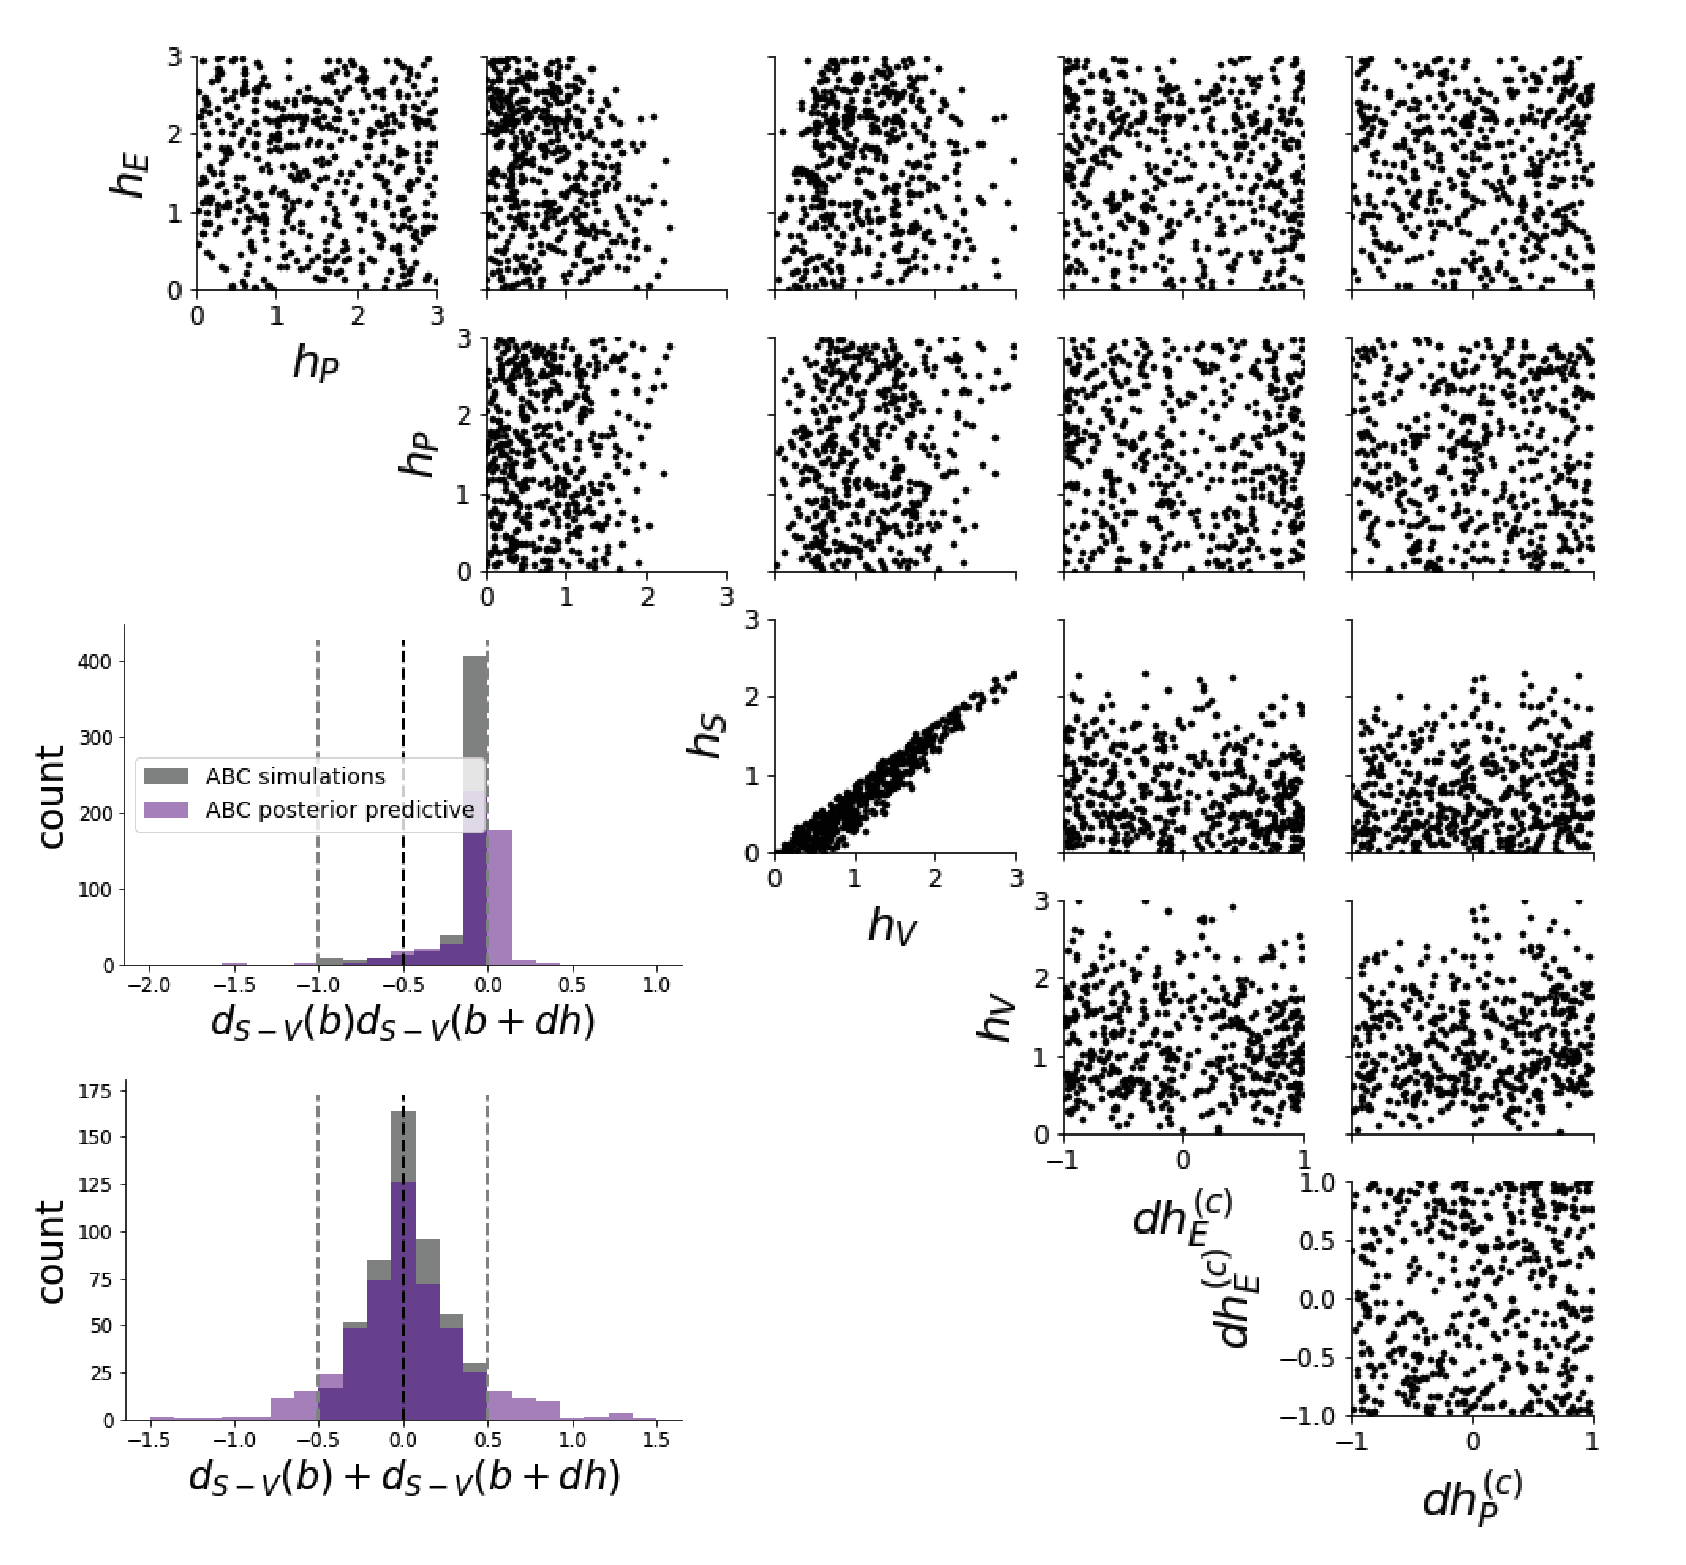
\includegraphics[scale=.3]{figs/FigSabc/FigSabc.pdf}
\end{center}
\end{figure}


\begin{figure}[h]
\caption{\small \textbf{A}. ...
 }\label{fig:drdh}
\begin{center}
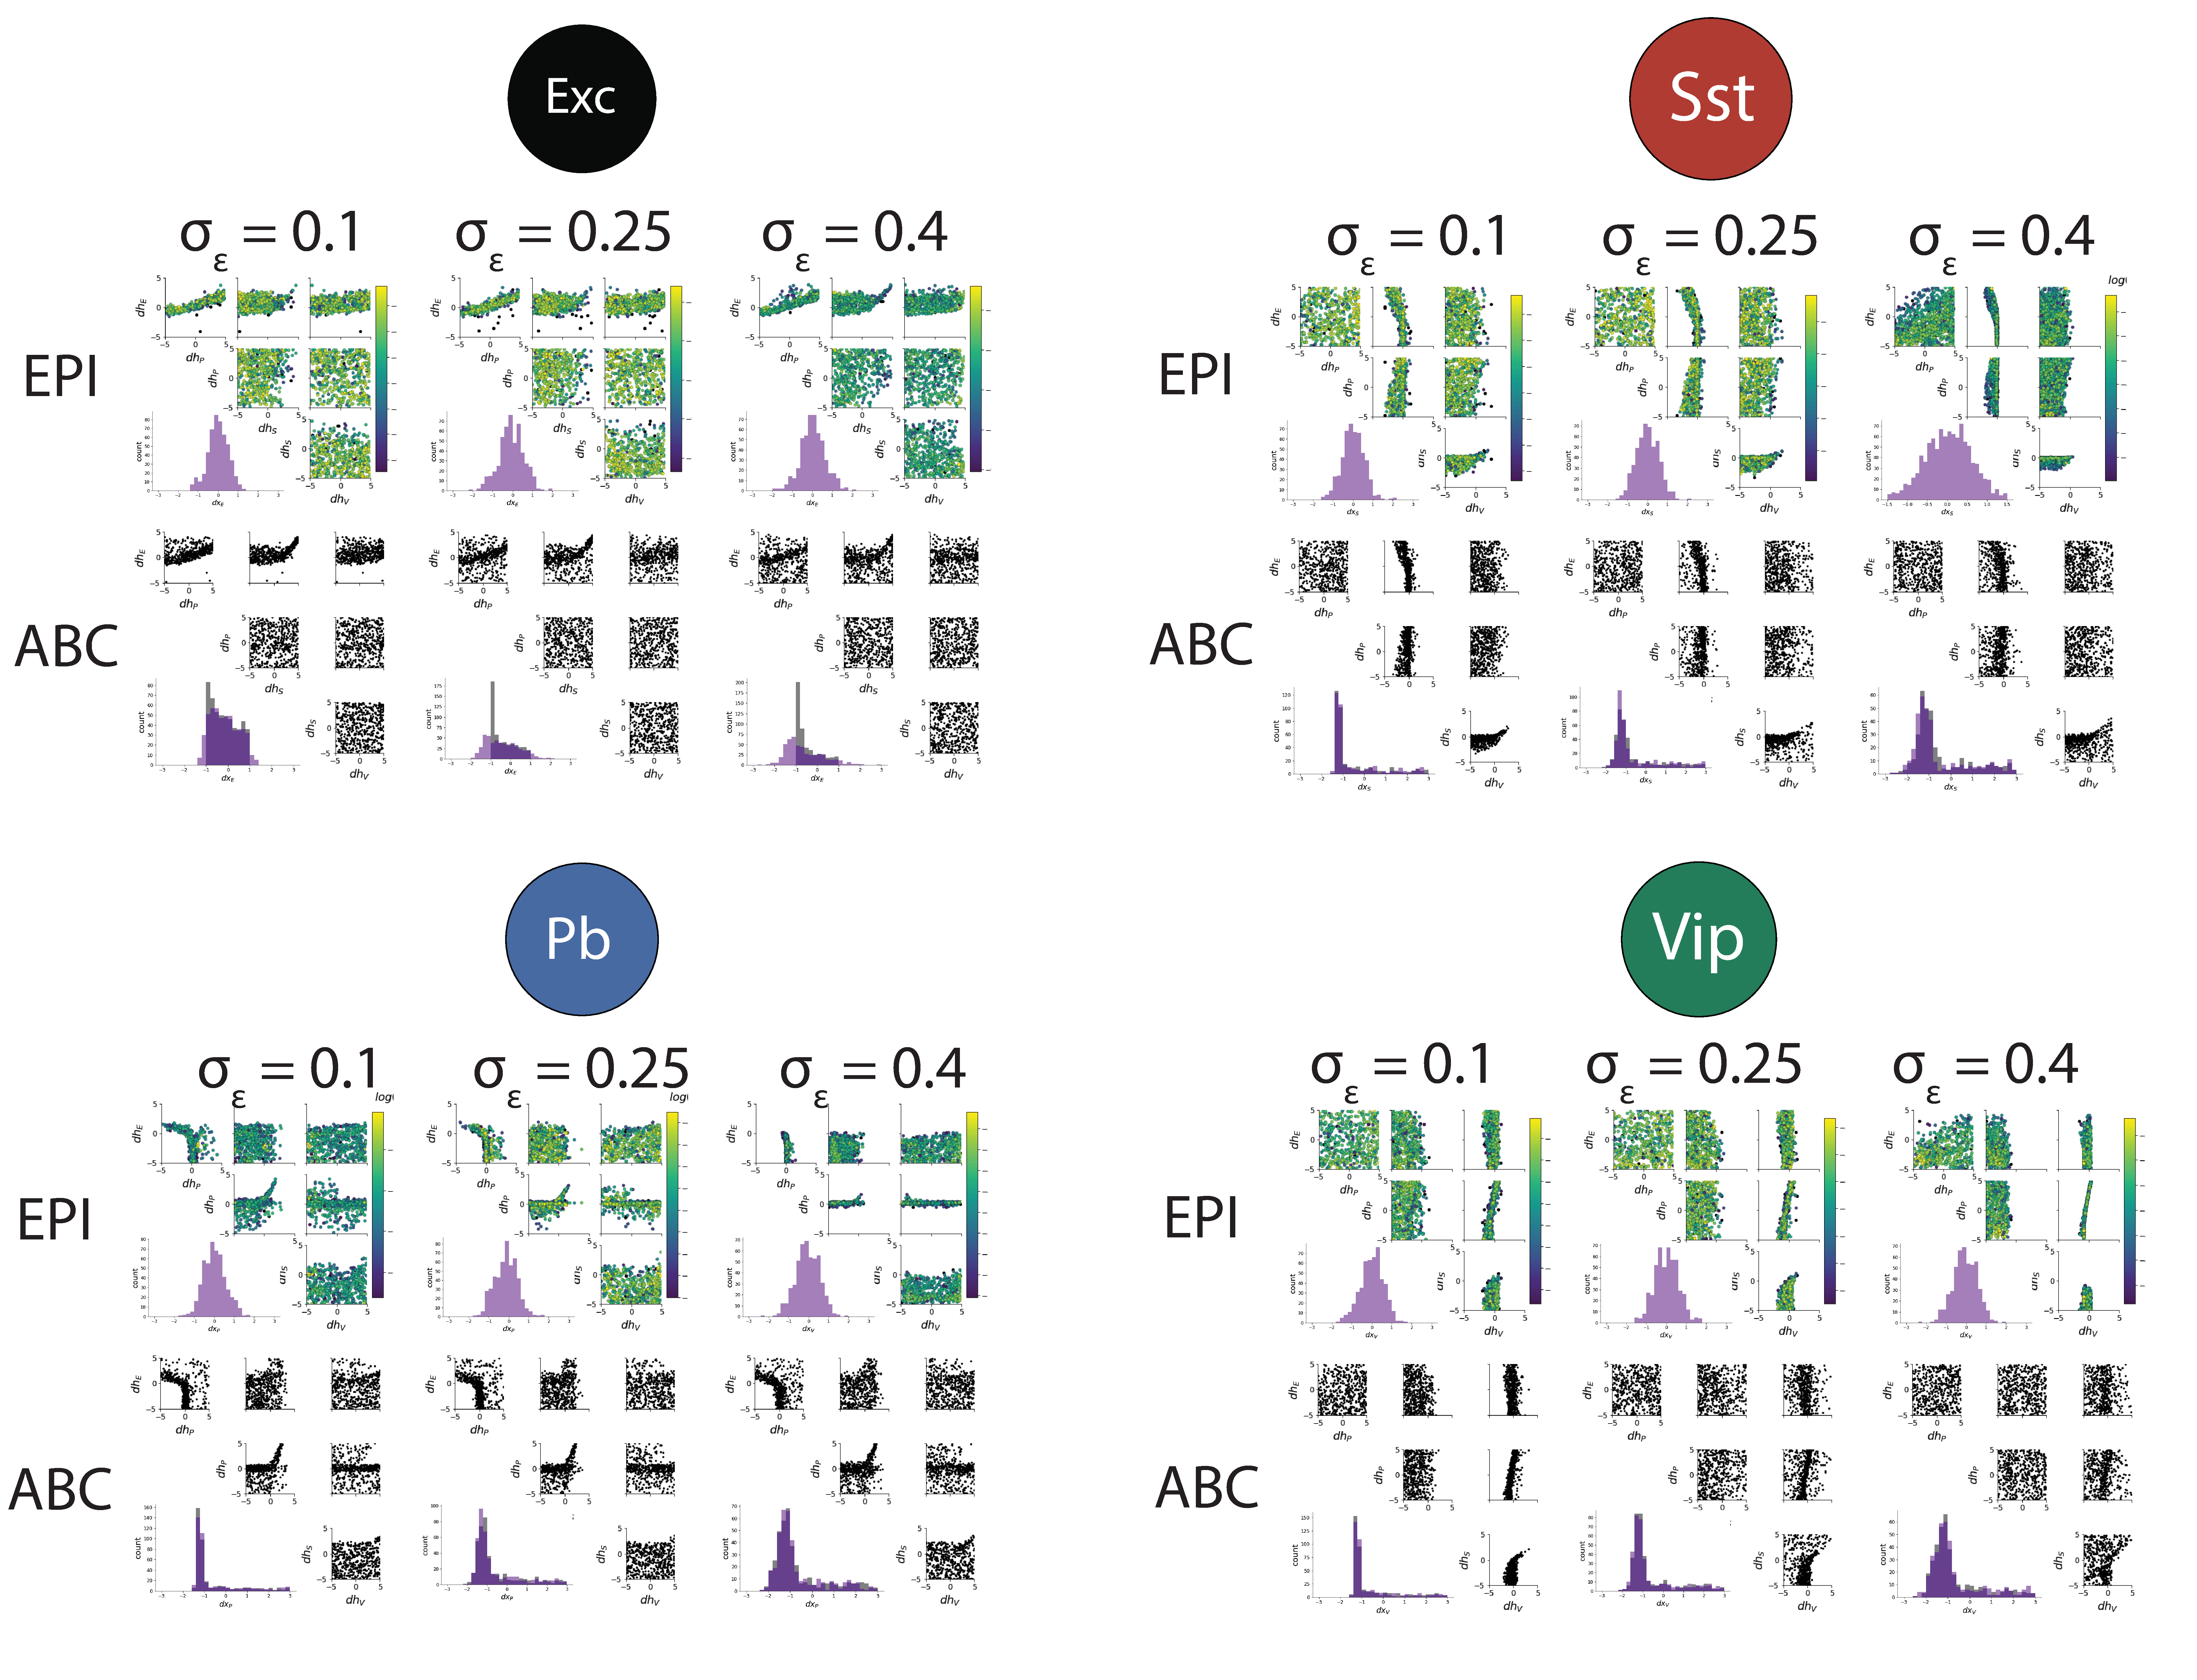
\includegraphics[scale=.12]{figs/FigSX/FigSX.pdf}
\end{center}
\end{figure}


\bibliography{epi}
\bibliographystyle{unsrt}

\end{document}

